\section{Наложение частот}
Как мы уже говорили, в реальности нам приходится работать не с непрерывными функциями, а с дискретизированными сигналами. Понятно, что дискретизация должна происходить с какой-то частотой. Назовем эту частоту $\omega_S = \frac{2\pi}{\Delta}$, где $\Delta$ - период дискретизации. Идеальная дискретизирующая функция может быть описана рядом:
\begin{equation}
    i(t) = \sum \limits_{n = - \infty}^{+\infty} \delta\left(t - n\Delta\right)
    \label{eq:tact}
\end{equation}

Это можно интерпретировать так: через каждые $\Delta$ секунд происходит измерение нашего сигнала. Таким образом в совокупности с измеряемым сигналом на выходе мы увидим дискретную функцию, которую можно описать следующим выражением:
\begin{equation}
    s_i(t) = s(t)\cdot i(t) = s(t)\sum \limits_{n = - \infty}^{+\infty} \delta\left(t - n\Delta\right)
    \label{eq:discreted}
\end{equation}

Давайте найдем ее Фурье образ. Для этого предлагаю сначала взять Фурье образ для выражения \eqref{eq:tact}, поскольку далее мы сможем с легкостью воспользоваться свойством свертки.
Но поиск Фурье образа \eqref{eq:tact} с ходу приводит к затруднениям, поэтому можно попытаться сначала разложить ее в ряд Фурье:
\[i(t) = \frac{1}{\Delta}\sum \limits_{k = -\infty}^{+\infty} C_k e^{\frac{2\pi kt}{\Delta}}\]
коэффициенты этого ряда нетрудно ищутся:
\[C_k = \int \limits_{-\frac{\Delta}{2}}^{\frac{\Delta}{2}}e^{\frac{2\pi kt}{\Delta}}\sum \limits_{n = - \infty}^{+\infty} \delta\left(t - n\Delta\right)\,dt\]
так как в пределах интегрирования находится всего лишь одна точка с $n = 0$, то по свойству дельта функции получаем $C_k = 1$ и ряд Фурье для функции \eqref{eq:tact} выглядит следующим образом:
\begin{equation}
    i(t) = \frac{1}{\Delta}\sum \limits_{k = -\infty}^{+\infty} e^{\frac{2\pi kt}{\Delta}}
    \label{eq:Fourier_series_tact}
\end{equation}
Теперь вспомним, что  $\delta(t)\xrightarrow{\mathscr{F}}1$ и, соответственно, наоборот.
Учитывая это получаем, что:
\begin{equation}
    i(t)  \xrightarrow{\mathscr{F}} \frac{1}{\Delta}\int \limits_{-\infty}^{+\infty} \sum \limits_{n = \infty}^{+\infty} e^{-2\pi i \left(\omega - \frac{n}{\Delta}\right)}\,dt =
    \frac{1}{\Delta}\sum \limits_{n = -\infty}^{+\infty} \delta\left(\omega - \frac{n}{\Delta}\right) = I(\omega)
\label{eq:i_fourier}
\end{equation}
Учитывая, что $s_i(t) = s(t)\cdot i(t)$, то по теореме свертки Фурье образ $S_i(\omega)$:
\[S_i(\omega) = \int \limits_{-\infty}^{+\infty}S(\omega - g) I(g)\,dg\]
Подставляя \eqref{eq:i_fourier} в эту формулу, получаем:
\begin{equation}
    S_i(\omega) = \frac1{\Delta}\sum \limits_{n = -\infty}^{+\infty}S\left(\omega - \frac{n}{\Delta}\right)
\label{eq:Fourier_Si}
\end{equation}
Таким образом, зная Фурье образ для функции $s(t)$, можем утверждать, что результирующий Фурье образ будет представлять собой наложение Фурье образов $s(t)$ через каждые $\frac{1}{\Delta}$ Гц. (Надо сделать рисунок).

Отсюда видим, что наложение спектров будет зависеть от величины $\Delta$. 

Здесь мы подходим к главному принципу --- поскольку функции дискретны и кончены из-за не бесконечного периода измерений, то чем шире в одном пространстве изображение функции (временном), тем уже ее изображение в другом пространстве (частотном). Поэтому период дискретизации следует уменьшать до тех пор, пока разрешение частот (отношение $\frac1{\Delta}$) не позволит нам различать периодические структуры друг от друга.

Также необходимо отметить, что для любой реально существующей функции Фурье образ является спадающей по частоте функцией. С физической точки зрения мы можем объяснить это так: каждая частота соответствует какой-то энергии. Чем больше частота, тем больше энергия, а, как мы знаем, бесконечной энергия быть не может, следовательно и Фурье образ стремится к нулю на бесконечности для любой функции.

\section{Проблемы прямоугольного окна. Размытие спектральных составляющих.}

Как мы убедились с помощью рисунка \ref{fig:rect_1}, прямоугольное окно преобразует совокупность синусоидальных сигналов совсем не в три дельта функции, как было бы в идеале. На деле же мы видим некоторые дополнительные частоты, вклад которых, хоть и мал, но присутствует в достаточно большом (я бы даже сказал в бесконечном) диапазоне. Внимательные из вас могли догадаться (это, кстати, говорилось ранее), что данный факт связан с крутизной фронтов временного окна, то есть в результирующем спектре наблюдаются высокие частоты, отвечающие за формирование <<резких>> краев наших ворот. 

Поэтому, как правило, в качестве ворот берется функция, которая внешне очень похожа на распределение Ферми-Дирака и задается следующей формулой:
\[w(t) = \frac1{\exp\left(\frac{|t| - T}{\sigma}\right) + 1}\]
здесь параметр $T$ - отвечает за длительность ворот, $\sigma$ - за крутизну фронта. Если построить график этой функции, то можно убедиться, что единственное отличие ее от прямоугольных ворот в крутизне фронтов, поэтому варьируя ее параметры можно добиться отсутствия нежелательных высоких и низких частот. 

Чтобы еще раз показать, что крутизна фронтов действительно влияет на результирующий спектр именно таким образом, приведу рисунок \ref{fig:gaus_separation}, аналогичный \ref{fig:rect_1}, только здесь в качестве временного окна используется функция гаусса. Несмотря на то, что это не похоже на приведенную выше функцию, однако фронты все равно позволяют наблюдать тенденцию уменьшения влияния высоких частот в отличие от случая использования прямоугольного временного окна.

\begin{figure}
    \centering
    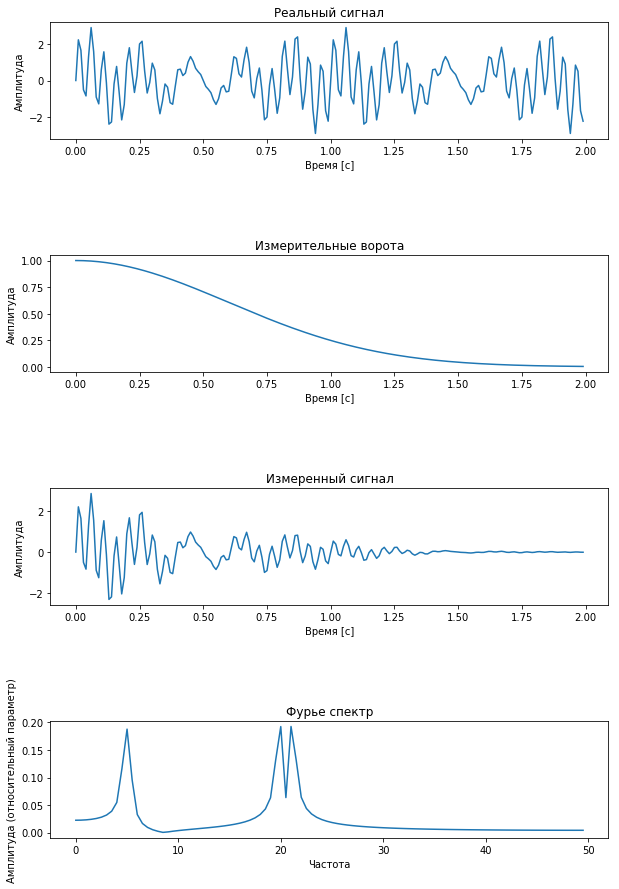
\includegraphics[scale = 0.5]{Pictures/separation_gaus.png}
    \caption{Использование временных ворот с менее крутыми фронтами.}
    \label{fig:gaus_separation}
\end{figure}
